\documentclass[10pt,a4paper,titlepage]{article}
\usepackage[utf8]{inputenc}
\usepackage{amsmath}
\usepackage{amsfonts}
\usepackage[T1]{fontenc}
\usepackage{graphicx}
\usepackage{csvsimple}
\usepackage{pdfpages}
\usepackage{float}
\usepackage[margin=2.5cm]{geometry}
\setlength{\parindent}{0in}
\author{Helen Harman \\ Student Number : 110007212 \\ Computer Science Department, Aberystwyth University}
\title{SE31520 Assignment : Enhancing the CS-Alumni Application}

\begin{document}

\maketitle 

\tableofcontents

\pagebreak 
\section{Introduction}
This document describes the workings of the CSA application. A detailed test plan for doing performing cucumber testing on the application has been given.
\section{Requirements Analysis}
I have not changed the functionality of the CSA application, so see Loftus \cite[5]{design} for a class diagram for CSA.

\subsection{Use Case Diagrams}
I have created several use case diagrams to show the current functionality that has been implemented within the CSA application. 
\subsubsection{Broadcasts}
\begin{figure}[H]
\begin{center}
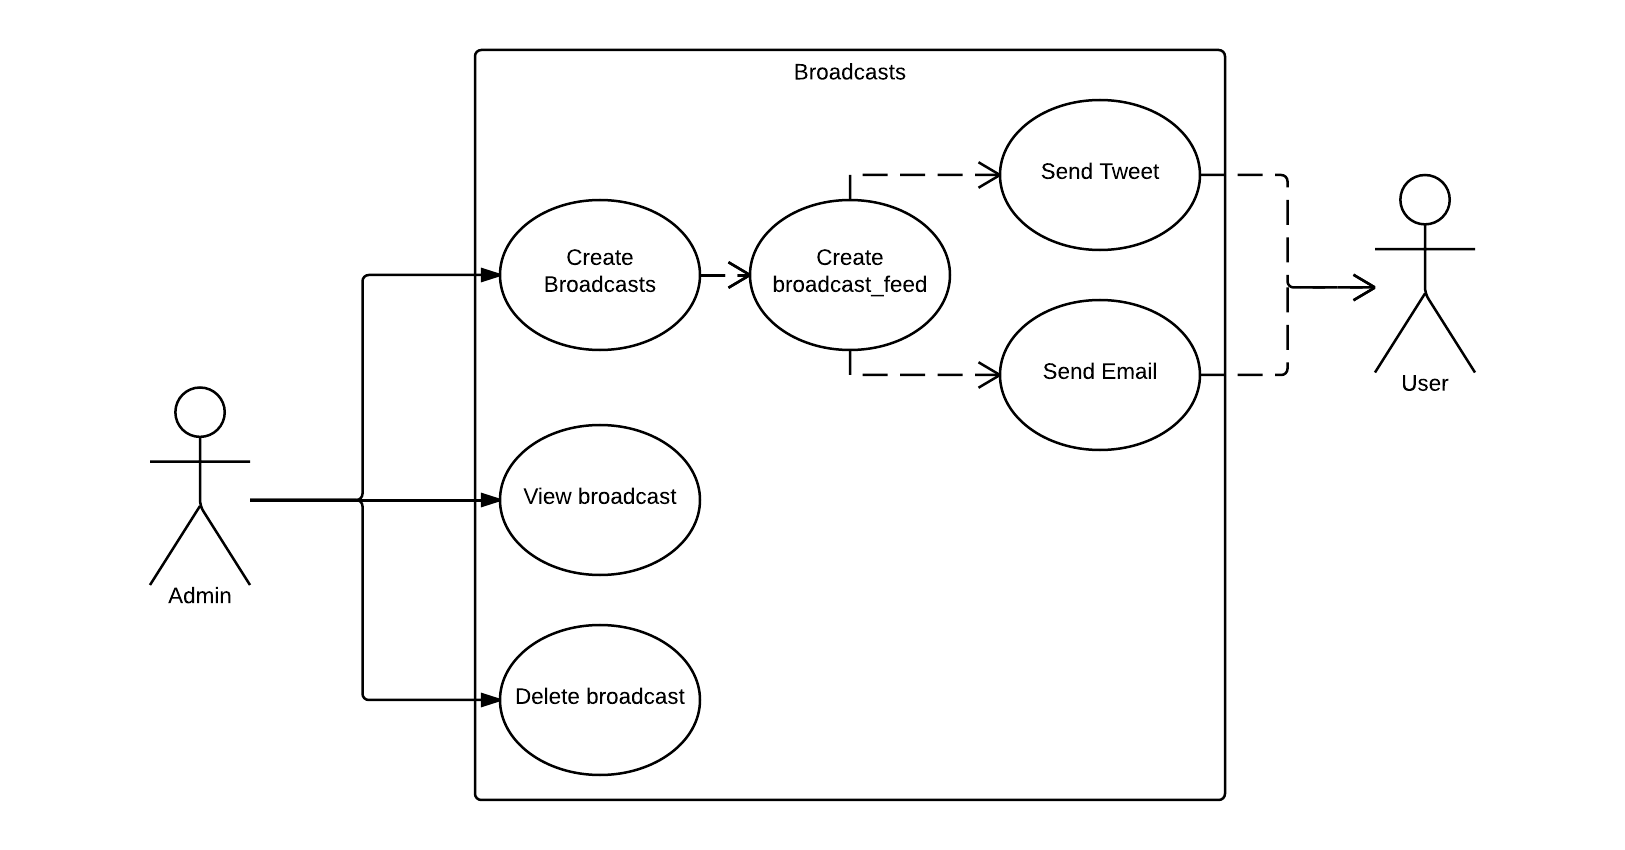
\includegraphics[scale=0.3]{include/broadcasts_Use_Case.png}  
\caption{Architecture : Use case for broadcasts. }
\label{fig:broadcastUseCase}
\end{center}
\end{figure}

An admin user should be able to :
\begin{itemize}
\item Create any number of broadcasts. This will be broadcast to multiple feeds, including Email and Twitter. A user will then receive the broadcast in an email or view the tweet. The admin will choose which feeds they wish to broadcast too.
	\begin{itemize}
	\item A user will receive the broadcast email and be able to view the Tweet. 
	\end{itemize}
\item An admin should be able to view the list of broadcast, and view a particular broadcast's content.
\item An admin should be able to delete a broadcast.
\end{itemize}
The admin will interact with the view part of the application, and any other the above actions will update the model with the correct data.

\subsubsection{User}
\begin{figure}[H]
\begin{center}
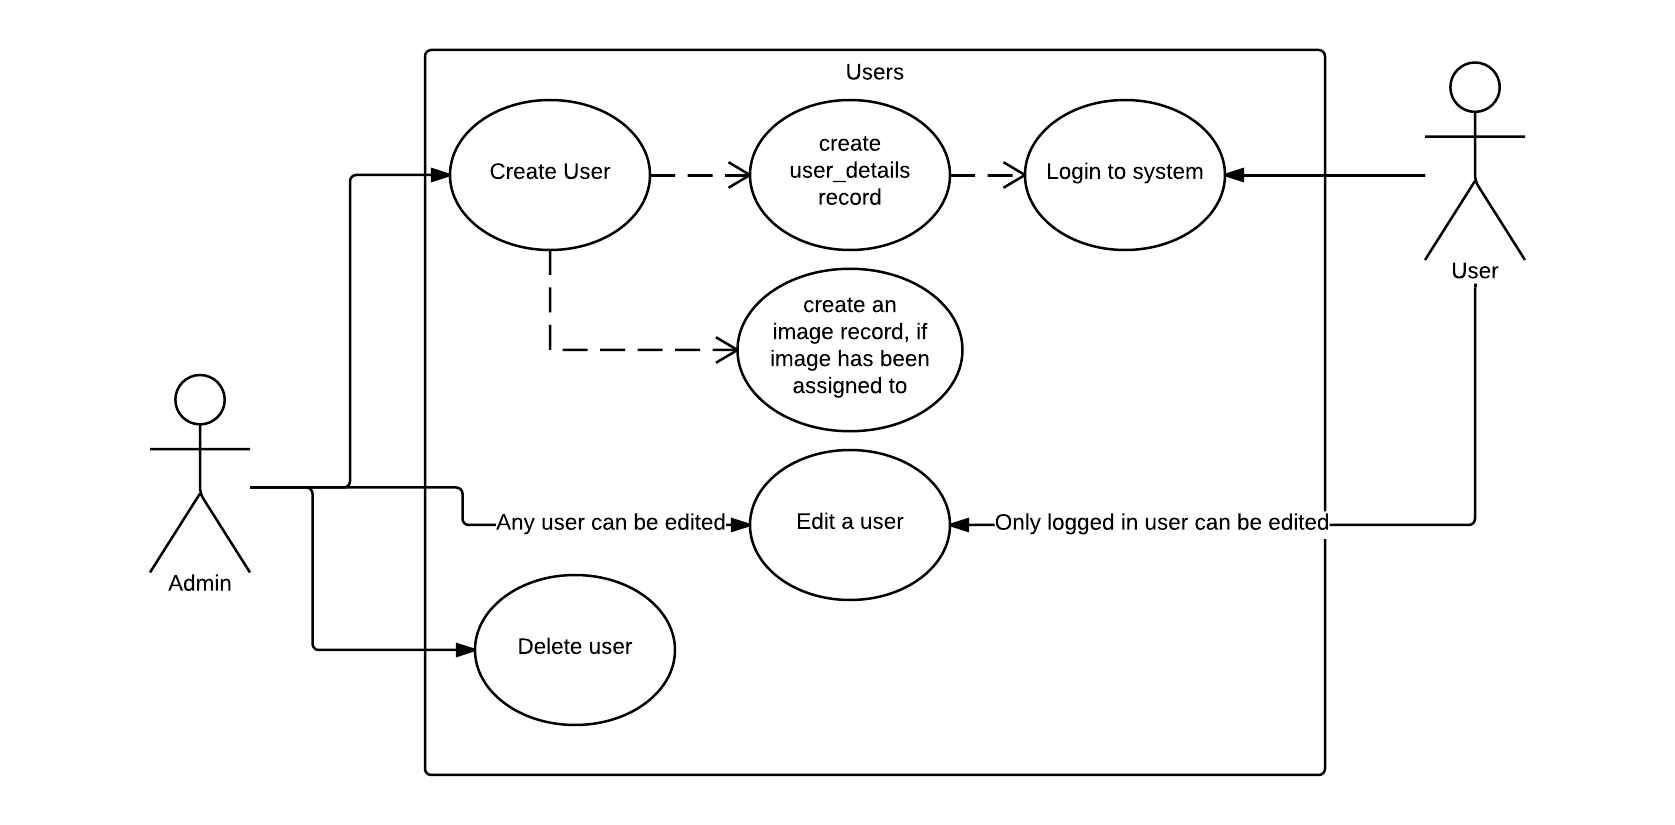
\includegraphics[scale=0.3]{include/User_Use_Case.png}  
\caption{Architecture : Use case for users. }
\label{fig:userUseCase}
\end{center}
\end{figure}

\begin{itemize}
\item The admin should be able to create a user, using a form. Doing this will create a record in the UserDetails model and a if an image is being used a record to the image model will be added. 
	\begin{itemize}
	\item A user will then be able to login to the application using the UserDetails the admin has entered.
	\end{itemize} 
\item An admin should be able to edit any of the users within the application using the web page. A user should only be able to edit their own account.
\item An admin should be able to delete a user.
\end{itemize}

\subsection{State Diagram}
\begin{figure}[H]
\begin{center}
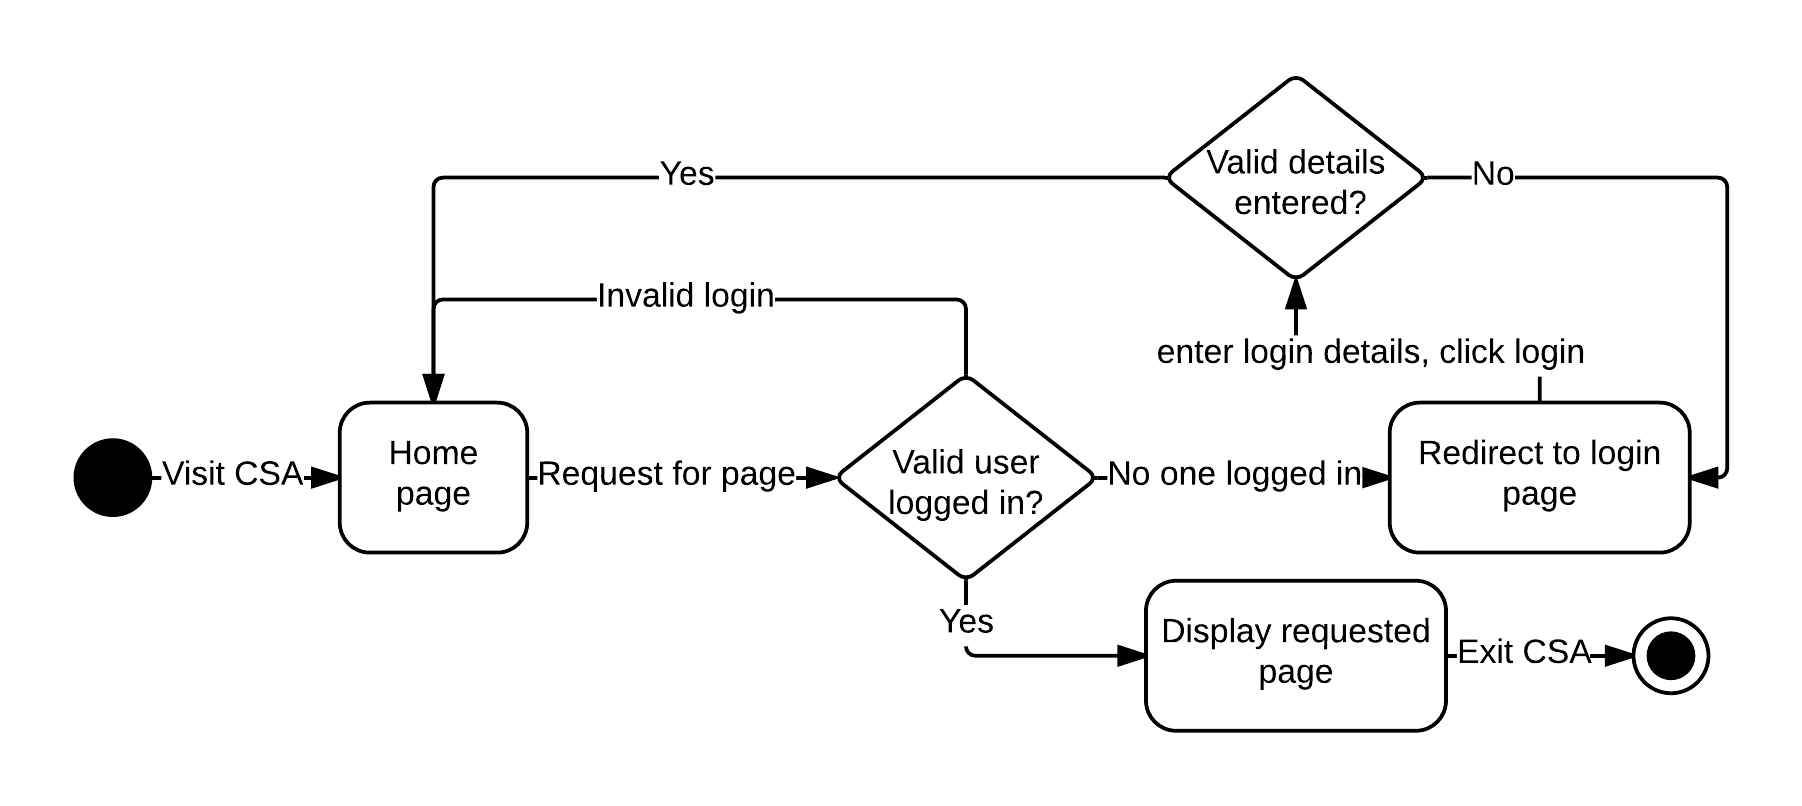
\includegraphics[scale=0.25]{include/State_Diagram.png}  
\caption{Architecture : State diagram. }
\label{fig:stateDiagram}
\end{center}
\end{figure}

The state diagram in figure~\ref{fig:stateDiagram} shows the state of the system when a user accesses the CSA application, requests a page and logs into the application. 

\section{Design}
\subsection{Class Diagram}
\begin{figure}[H]
\begin{center}
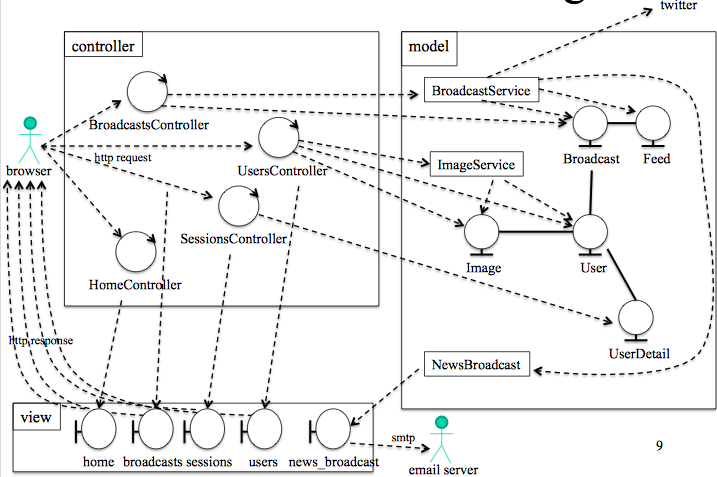
\includegraphics[scale=0.55]{include/classDiagram.png}  
\caption{Design : Class diagram. This class diagram was produced by Loftus\cite[5]{design}}.
\label{fig:classDiagram}
\end{center}
\end{figure}
When a client/browser sends a request to the CSA application, the request gets sent to the controller. 
\begin{itemize}
\item In the case of the Home page, then HomeController gets run and the home view gets sent as a HTTP response to the client. 
\item When a client requests to be logged in (or is logged in) their request gets sent to the SessionsController. The userDetails in the session parameters are compared to those in the UserDetail model. If the login details are correct then the sessions view is given as a HTTP response to the client/browser. 
\item When a users page is requested the UsersController accesses the Image and User model to get the data for the user(s), the users view is then sent to the browser as a HTTP response. 
\item When a broadcast is posted to the BroadcastsController a record in the broadcast model is added. BroadcastServices is used to process broadcasting the broadcast to the different feeds. A feed record is created for each type of feed the broadcast is being sent to. 
	\begin{itemize}
	\item When an email being created the content of the email is entered into the news\_broadcast and SMTP is used to send the email to the users.
	\end{itemize}
	
\end{itemize}
\section{Test Strategy}
For the addition I made to the application I decided to add cucumber tests using capybara and selenium. This way I could see what parts of the application are yet to be implemented, what improves could be made. Have a full set of tests before changing an application is important, as you do not want to break any of the current system. 

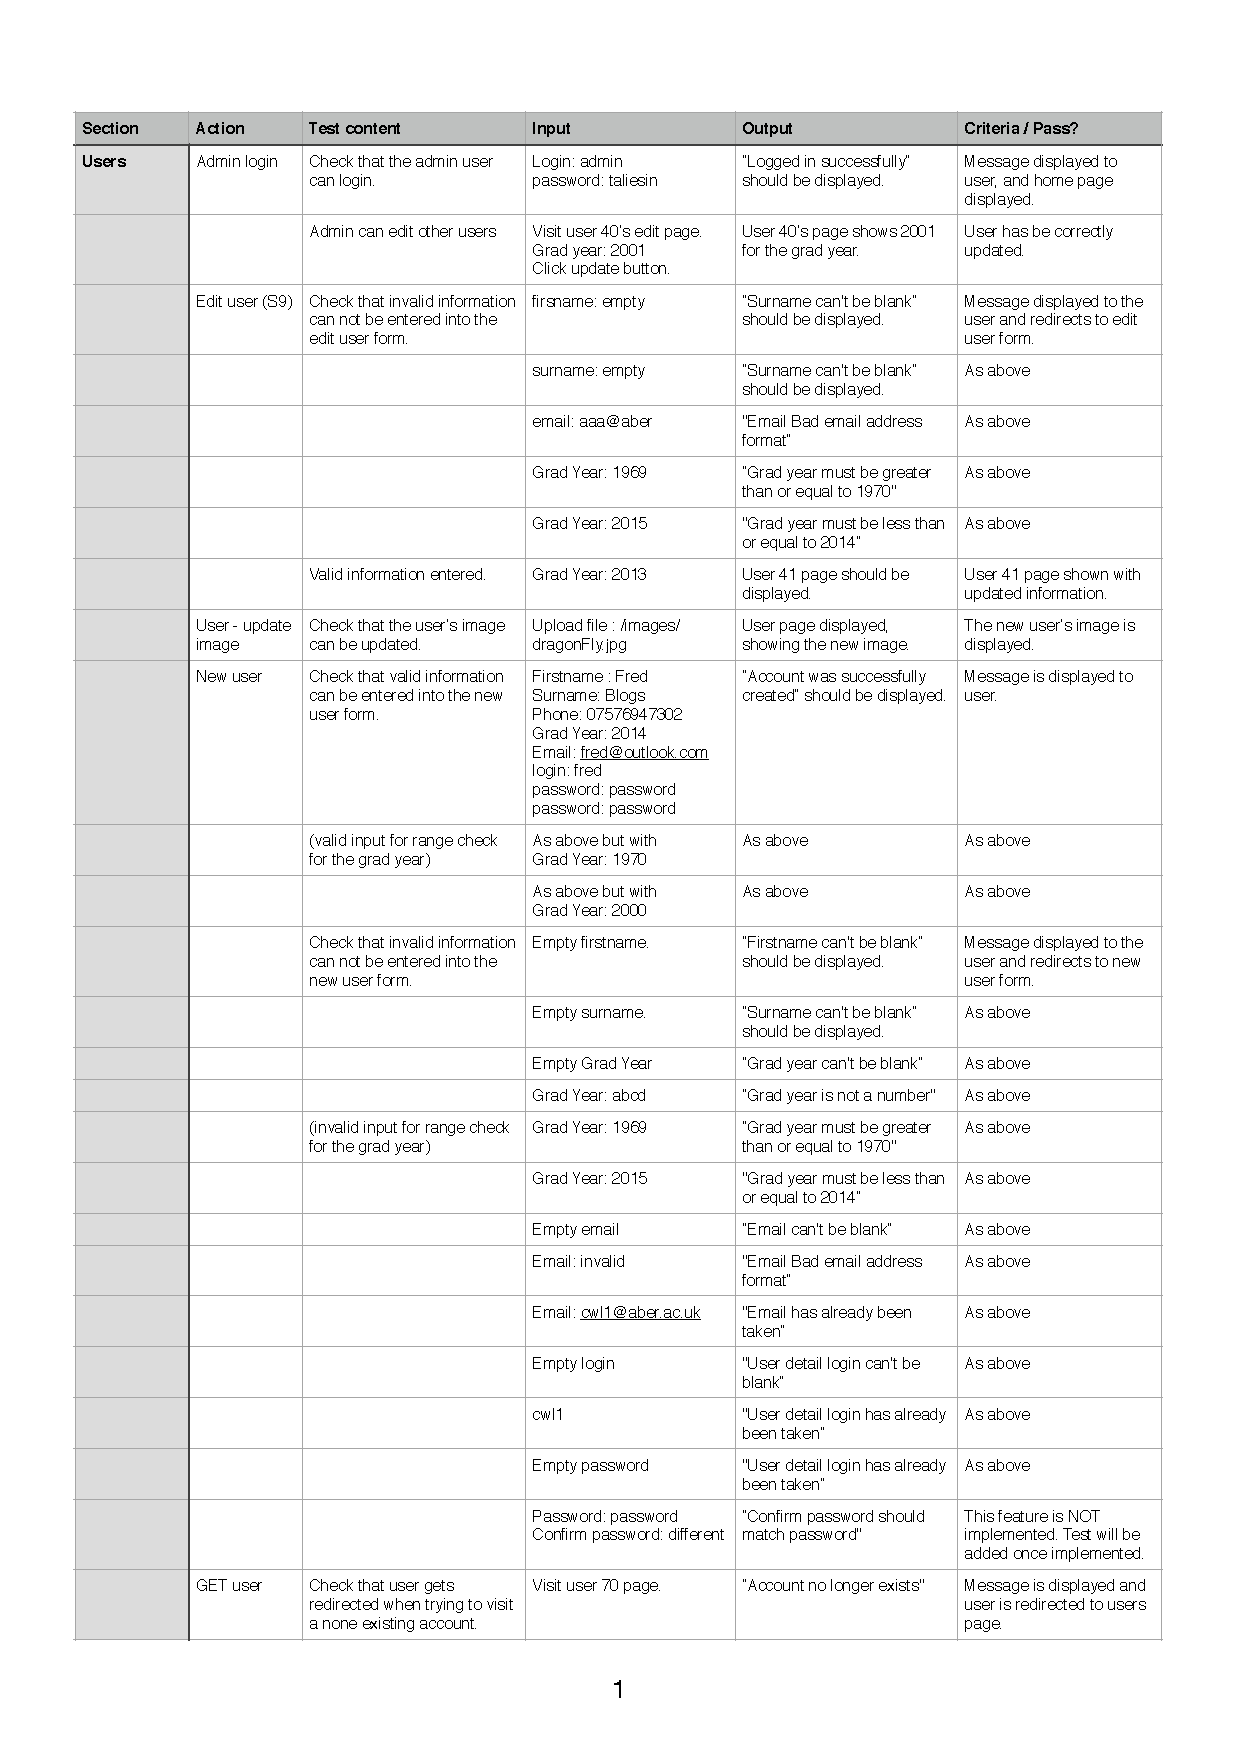
\includepdf[pages={1-3}]{include/testTable.pdf} 

\subsection{A few of the issues found}
\begin{itemize}
\item While logged in as an admin, you can delete the admin user.
\item The "Shorten URL" on the broadcasts page does not do anything.
\item The confirm password field does not have any validation. It can be different from the password.
\end{itemize}


\subsection{Script To Execute Tests}
I have created a python script that executes the cucumber tests; saves the results to a database (testResults.db) and  plots a graph to show the test results over time. This has been used to show the progress made while creating tests and the amount of code these tests are covering. Showing progress often helps to keep developers more focused.\\

The sequence diagram in figure~\ref{fig:sequenceDiagram} shows how this script works.

\begin{figure}[H]
\begin{center}
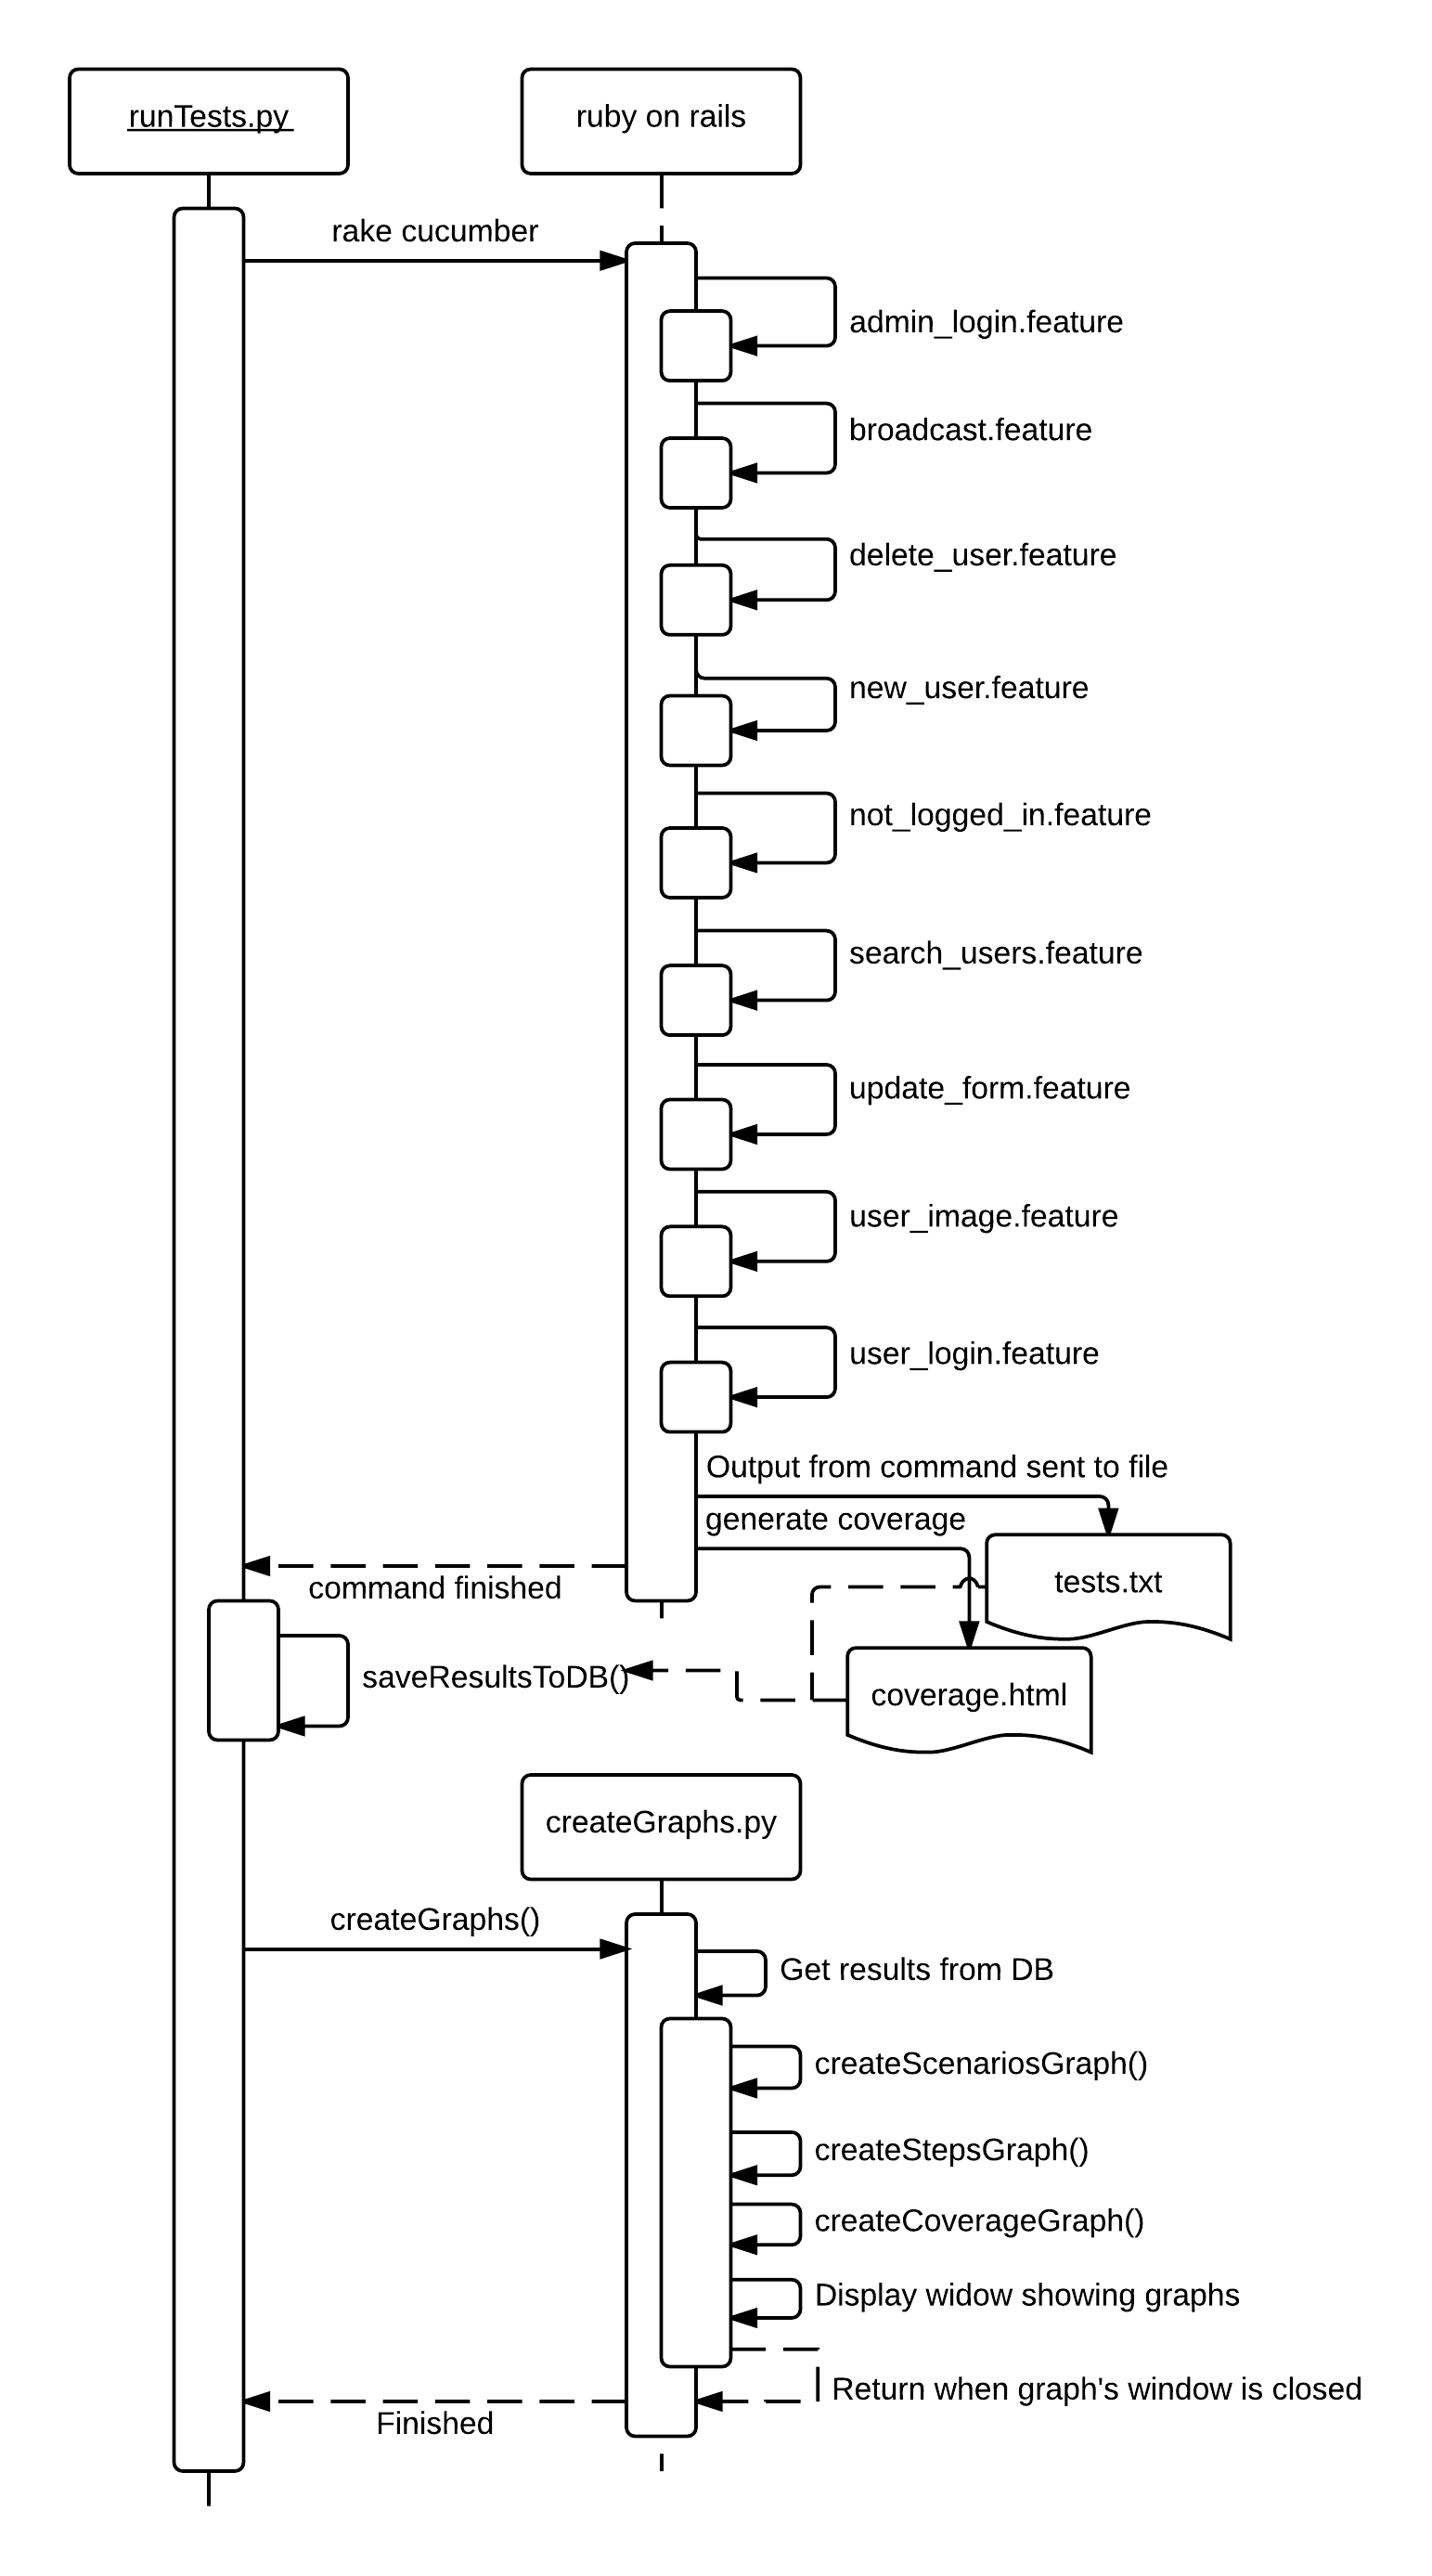
\includegraphics[scale=0.25]{include/Sequence_Diagram.png}  
\caption{Test Strategy : Sequence Diagram. }
\label{fig:sequenceDiagram}
\end{center}
\end{figure}
I also created the following support files:
\begin{itemize}
\item env.rb
	\begin{itemize}
	\item Runs the seed.rb file to fill the test database with the same data as the development database. The database gets cleaned between each of the scenarios. 
	\item Sets up the fillers and groups for the simpleCov to be run.
	\end{itemize}
\item paths.rb
	\begin{itemize}
	\item Gets the path to the given page. Where page is the string from the feature. This is used to visit a page and to check that the current page is correct.
	\end{itemize}
\item search\_helper.rb
	\begin{itemize}
	\item Used to fill in the search filled, and select an item from the drop down menu.
	\end{itemize}
\item helper.rb
	\begin{itemize}
	\item Any addition functions that are needed. Currently just contains function to get the current time.
	\end{itemize}
\end{itemize}

\subsection{Test Results}

Figure~\ref{fig:graphOutput},~\ref{fig:cucumberOutput} and~\ref{fig:coverageOutput} show the output from running the cucumber tests. As you can see from the figures 31 scenarios with 385 steps have been run. These have managed to cover 87.5\% off the CSA application. It would be hard to increase the coverage any further, with the current implementation.

\begin{figure}[H]
\begin{center}
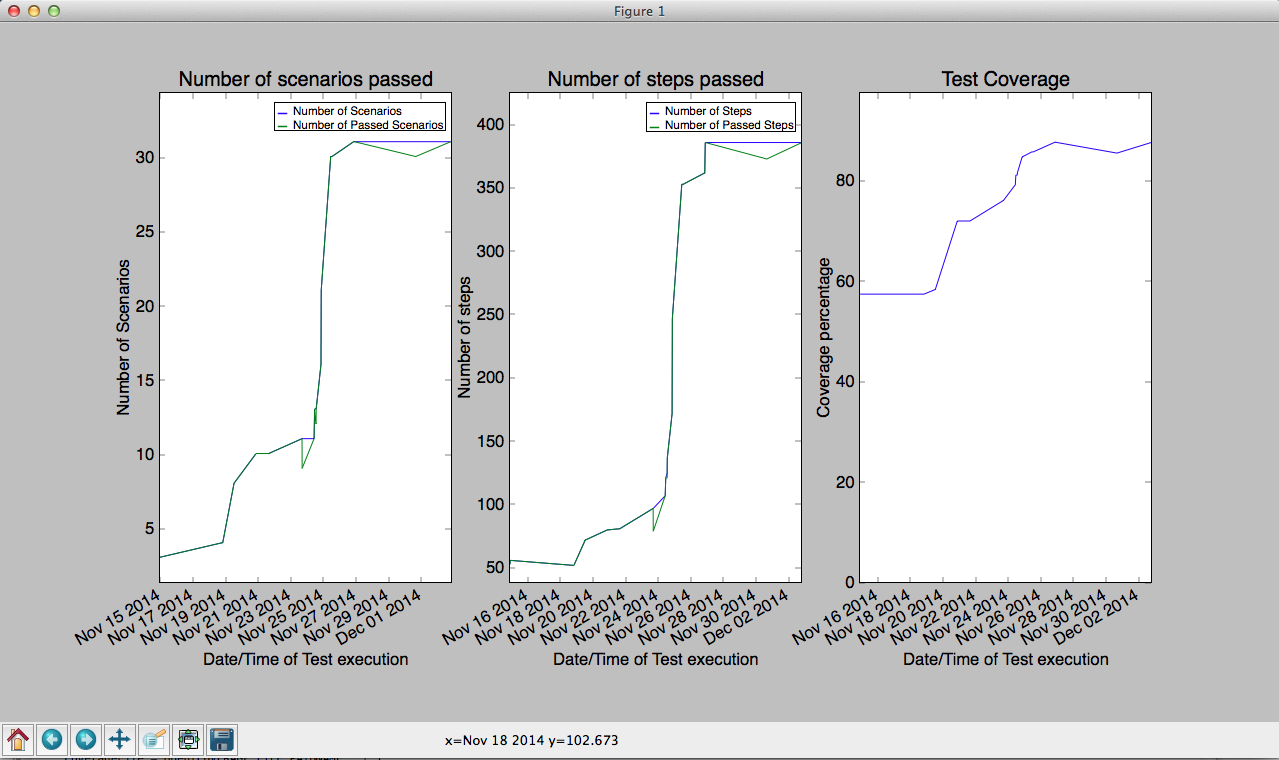
\includegraphics[scale=0.35]{include/graphOutput.png}  
\caption{Test Results : Output from running the python test runner. }
\label{fig:graphOutput}
\end{center}
\end{figure}

\begin{figure}[H]
\begin{center}
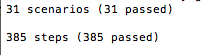
\includegraphics[scale=1.0]{include/cucumber_results.png}  
\caption{Test Results : The scenarios and steps that have been run. }
\label{fig:cucumberOutput}
\end{center}
\end{figure}

The output shown in figure~\ref{fig:coverageOutput} is produced by the simpleCov gem. My tests manage to cover 87.5\% of the code in the CSA application. 

\begin{figure}[H]
\begin{center}
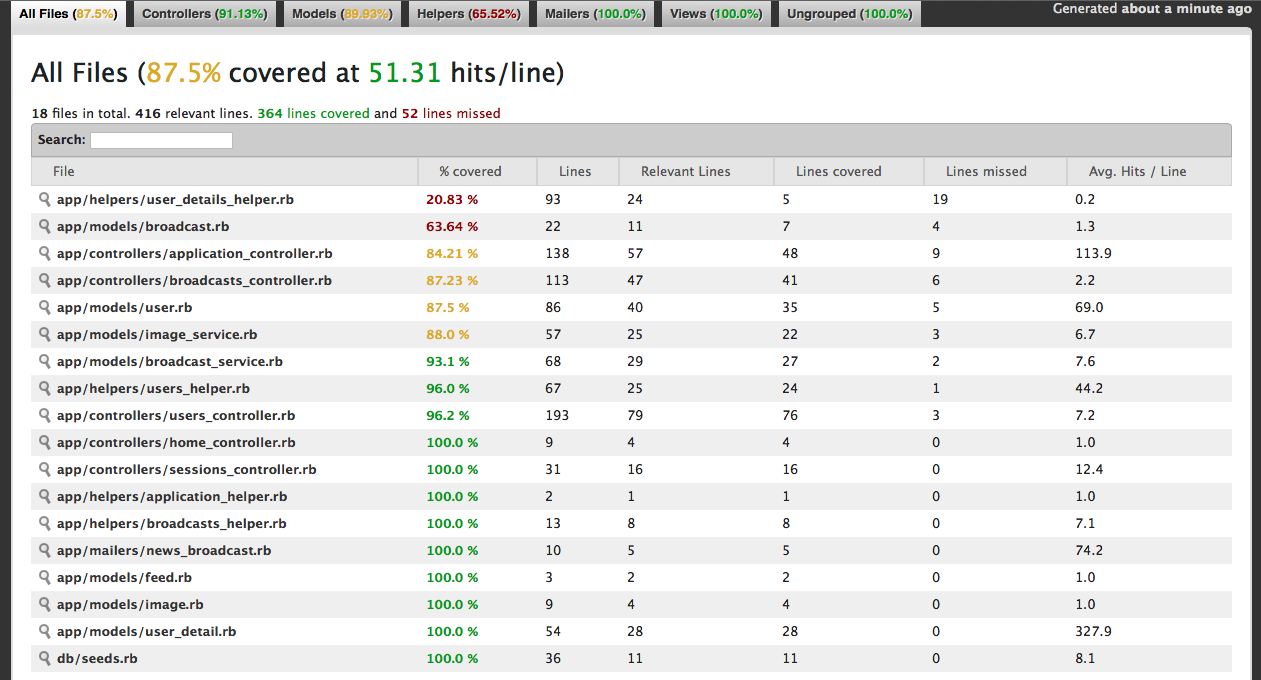
\includegraphics[scale=0.35]{include/coverage.png}  
\caption{Test Results : The output produced by the coverage gem. }
\label{fig:coverageOutput}
\end{center}
\end{figure}

\section{Critical Evaluation}

Before the start of this module I had never had any experience with ruby or much experience with different web technologies. I took me awhile to learn these new technologies and to find my way around the CSA application. I also had to learn about cucumber testing, and found it strange to work in a behaviour driven way. Once I had gotten use to writing features then developing the tests became a lot quicker. Learning the technologies meant that I spent a lot longer on the assignment than the recommended 50 hours.\\

I have had some past experience with python but had not used the matpotlib before so wanted to gain experience of using this module. Creating the graphs gave me this experience. The Python scripts could then easily be started from a continuous integration sever like Jenkins/Hudson.\\

I would give the following marks to each section:
\begin{itemize}
\item Successfully running the provided CSA prototype : 4\%
	\begin{itemize}
	\item I have included a screencast showing the working CSA application. 
	\end{itemize}
\item Design and documentation (Cucumber test project): 10\%
	\begin{itemize}
	\item Design lacks some details, but range of diagrams used to show how the applications works.
	\end{itemize}
\item Implementation: 25\%
	\begin{itemize}
	\item OK identifiers used, code is commented. Only one function in some helper files, so these could be combined.
	\end{itemize}
\item Flair: 9\%
	\begin{itemize}
	\item Included Python program that creates graphs of the results.
	\end{itemize}
\item Testing (Cucumber test project): 22\%
	\begin{itemize}
	\item Decent coverage percentage, test table included and test plan included. More details about the choice of tests could be included.
	\end{itemize}
\item Evaluation: 4\%
	\begin{itemize}
	\item Lots of details.
	\end{itemize}
With a total mark of 74\%

\end{itemize}



\subsection{Technologies Used}
\begin{itemize}
\item Ruby 2.1.3 - Programming Language
\item Rails 4.1.5 - Framework
\item SQLite3 - Database (including the test result database)
\item Cucumber - Testing gem using description of the behaviour of the application
\item Capybara-webkit - used to automate the cucumber tests.
\item Selenium-webdriver
\item JSON - used to check that a tweet has been created.
\item Javascript and AJAX - Used when performing the search for a user.
\item SimpleCov - Produces the HTML coverage, for running the cucumber tests.
\item Python - Create the graphs for the test results. matpotlib has been used.
\item SQLite3 - Used in setting up the test results database and when using the test database.
\end{itemize}

\subsection{Problems Encounter}
\begin{enumerate}
\item I had lots of issues getting the CSA application running. Eventually I found the places that the issues with the force SSL where happening, and commenting them out got the application running. 

\item When first running the cucumber tests I did not realise that it was running from the test database rather than development database. I spent a long time changing pieces of code until I realised that a admin couldn't login because they didn't exist in the database. 

\item Software, Framework and GEM Versions.\\
	While Googleing for solutions for many of the issues I had, I received many results that did not work for the versions of the software I am using.  
	\begin{itemize}
	\item I had a lot of issues with dealing with the pop-up received when a broadcast or user is deleted. I tried a lot of methods before finding one that works. 
	\item I had similar issues when trying to test the search for a user as AJAX had been used to perform the search.
	\end{itemize}

\item After installing ImageMagick uploading a image to the user still did not work. Later I found that this was because I did not have the path set to the correct place. 
	
\item Within the tests after posting the Tweet I then check that twitter has been updated with the tweet. I tried many different way to get this working. This included getting the page the Tweet is on, but this would be different for every tweet I create. In the end I just use the Twitter token to get the last tweet that the account created. This means that if another Tweet happens between the Tweet it creates and when I check it, the test will fail.

\item I also had issues with created the same tweet multiple times. Tweet does not allow a user to make the same tweet multiple times within a certain time frame. To solve this I added the time to the tweet. If the time (minutes/hours) changes between the creation of the tweet and the checking of the tweet, then the test will fail. Out of all the times I have run the tests this has only happened once. 	

\end{enumerate}
All of these problems are simple to solve once you know how, and most are fixed with just one or two lines of code.

\section{Attributions}

Additional Gems and rails related attributions:
\begin{enumerate}
\item Cucumber
\begin{itemize}
\item The instructions I used for using cucumber can be found at http://cukes.info/
\item To learn how to use cucumber I used the following tutorial: http://loudcoding.com/posts/quick-tutorial-starting-with-cucumber-and-capybara-bdd-on-rails-project/. Using paths.rb file was suggested by this tutorial.
\end{itemize}
\item I used Capybara API (http://www.rubydoc.info/github/jnicklas/capybara/Capybara/) while writing the steps.
\item Learnt the ruby regular expressions from http://www.agileforall.com/2010/07/just-enough-regular-expressions-for-cucumber/
\item I found the simpleCov gem at https://rubygems.org/gems/simplecov
\item I learnt how to upload files with cucumber using https://cassiomarques.wordpress.com/2009/01/23/how-to-test-file-uploads-with-cucumber/
\end{enumerate}

Other attributions:
	\begin{enumerate}
	\item All figures I have created have been formatted using http://lucidchart.com/ 
	\item When creating the python code I used http://matplotlib.org to learn how to use the matplotlib library.
	\end{enumerate}


\begin{thebibliography}{1}

\bibitem{design}Chris Loftus (2014), Requirements/Design for the CS-Alumni Application, [Online], Available: https://blackboard.aber.ac.uk/bbcswebdav/pid-487373-dt-content-rid-767088\_1/xid-767088\_1 [30 November 2014].



\end{thebibliography}

\end{document}